\chapter{Конструкторский раздел}
В данном разделе будут рассмотрена схема работы алгоритма конвейерной обработки, описание архитектуры ПО и схемы рабочего и главного процессов.

\section{Описание архитектуры ПО}
В конвейере 3 основные ленты, содержание их работы описано выше, в аналитической части отчета. Каждой ленте выделен свой поток, в котором она выполняется. В главном потоке (функция main) создаются три рабочих потока: по одному на каждую ленту.
Для каждой ленты есть своя очередь, однако с ней могут работать все потоки, поэтому при доступе к элементам очереди необходимо блокировать доступ для других потоков. Для реализации доступа из разных потоков используются мьютексы, по одному для каждой очереди и для результирующего массива.
Также в главном потоке генерируется массив входных данных и заполняется первая очередь (уровень 0). Для моделирования ситуации постепенного поступления данных, первая очередь заполняется с задержкой.
В рабочих процессах считывается по одному элементу из соответствующей очереди, выполняется вызов обрабатывающих функций, замеры времени и задержка по времени. После обработки текущей задачи, рабочий процесс записывает результат в следующую очередь или в результирующий массив. Также выполняется запись в лог—файл.
\section{Схема алгоритмов работы конвейерной обработки}
На рисунке \ref{png:conveyor_1} представлена схема алгоритма выполнения главного потока.
\begin{figure}[H]
	\centering{
		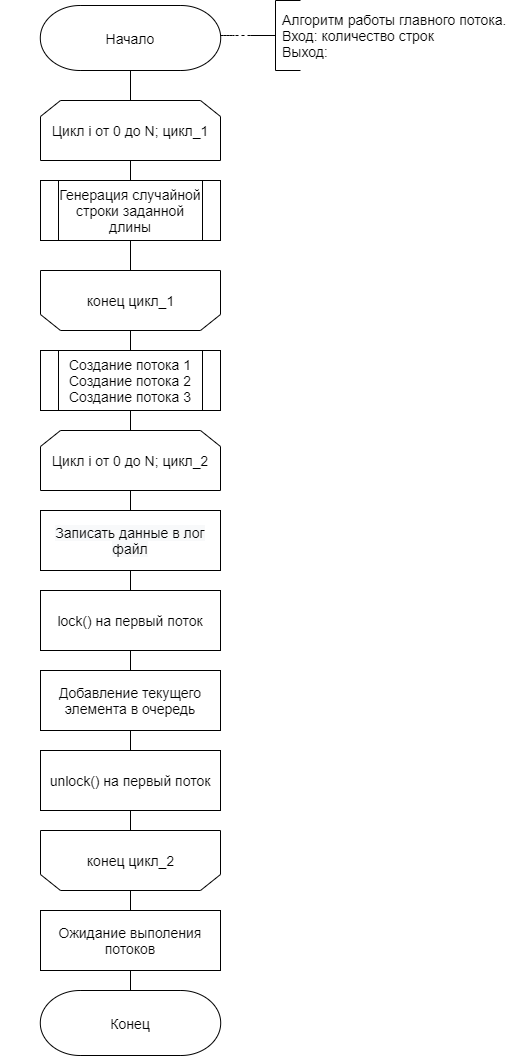
\includegraphics[scale=0.6]{../../../../../../../msys64/home/Лев/bmstu_sem_5_aa/lab_05/report/diagrams/conveyor_1}
		\caption{Схема алгоритма выполнения главного потока}
		\label{png:conveyor_1}
	}
\end{figure}
На рисунке \ref{png:conveyor_2} представлен схема алгоритма выполнения дочерних потоков.
\newpage
\begin{figure}[H]
	\centering{
		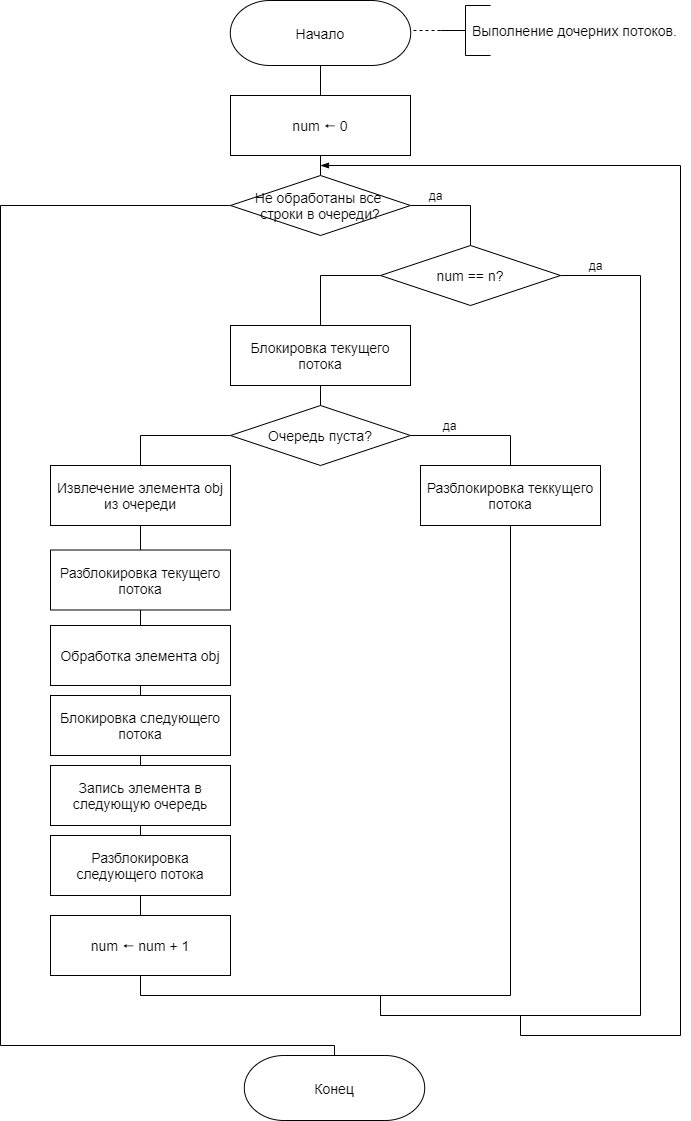
\includegraphics[scale=0.6]{../../../../../../../msys64/home/Лев/bmstu_sem_5_aa/lab_05/report/diagrams/conveyor_2}
		\caption{Схема алгоритма выполнения дочерних потоков}
		\label{png:conveyor_2}
	}
\end{figure}
\section{Классы эквивалентности}

Классы эквивалентности для тестирования:

\begin{itemize}
	\item пустые строки;
	\item количество строк на вход конвейера <= 0;
	\item строки из цифр, знаков препинания и других символов;
	\item корректные входные значения.
\end{itemize}

\section{Используемые типы данных}
В программе используются следующие типы данных:
\begin{itemize}
	\item строка - структура типа $input_t\_t$, являющимся переопределением типа std::string; 
	\item очереди имеют тип $std::queue<input\_t>$;
	\item переменные потоков thread1, thread2, thread3 - типа $std::thread$;
	\item время выполнения этапов обработки каждой матрицы записывается в переменные типа $clock\_t$ 
	\item для записи данных в файл используется тип $FILE *$;
	\item для исключения коллизий во время работы потоков применяются мьютексы $std::mutex$.
\end{itemize}


\section{Вывод}
В данном разделе была описана программа с 3 конвейерными потоками были приведены схемы алгоритмов используемых в программе описаны типы используемые в программе и классы эквивалентности для тестовых данных.